\chapter{Code Organization}

The code for this report is based off of Google's Verified Boot reference repository\cite{vboot-codebase} and the modifications can be accessed in a cloned and edited repository\cite{my-repo}.
Changes were to the Verified Boot repo were mostly restricted to the main Makefile and the unit test folder \code{tests/}.

In order to have the results reproducible, all work was done inside of Vagrant Virtual Machine running Fedora 23. 
To get a working environment, clone the repository, initialize the Vagrant box, and run the following command:
\begin{equation}
    \code{\$PATH/CBMC-Vboot/scripts/install-fedora.sh} 
\end{equation}
This script will install the 49 packages required to run all of the code. 
Next, restart the Vagrant box and run the initialization script with:
\begin{equation}
    \code{\$PATH/CBMC-Vboot/scripts/init-fedora.sh} 
\end{equation}
This script will compile the 6 packages that need specific configurations.

The installation process takes roughly an hour on my 2015 Macbook Pro and the resulting VM image requires 4 Gbs of Hard Drive space. 

The \code{scripts/} folder contains the configuration scripts.
The main scripts are for installation, but there are also scripts to manage the SW TPM library, and to build a Vboot Image with related Public/Private keys.

The \code{qemu/} folder contains all of the code to run Vboot within QEMU with the hardware setup described in Section~\ref{qemu_em}.
The \code{tpm-pcr.c} file tests the only the TPM PCR functionality.
The \code{tpm-badcmds.c} file stress tests the TPM behavior with bad commands.
The \code{vboot-full.c} goes through the full process of Chrome's Verified Boot.
The \code{README.md} file contains information on building the software and using GDB testing.

The \code{CBMC/} folder contains all of the code for running Formal Verification on Vboot.
The python files with the naming structure \code{run\_\{\$FILE\}.py} will build and run the CBMC command for \code{\$FILE}.
The C files with the naming structure \code{test\_\{\$FILE\}.c} contain the main code being tested by CBMC\@.
The \code{README.md} file contains information on repeating the tests outlined in this report.


\section{CBMC Command Builder}
The code below shows the python script that builds a CBMC command for Formal Verification.
\lstinputlisting[language=Python]{code/cbmc.py}

\section{TPM Firmware}
This code shows the TPM read and write functionality.
\lstinputlisting[language=C]{code/tpm.c}

\section{TPM ILA}
This code shows the ILA for the TPM Hardware
\lstinputlisting[language=Python]{code/TPM_ILA.py}

\chapter{Images and Charts} 

\section{Images}

\begin{figure}[!htbp]
  \centering
  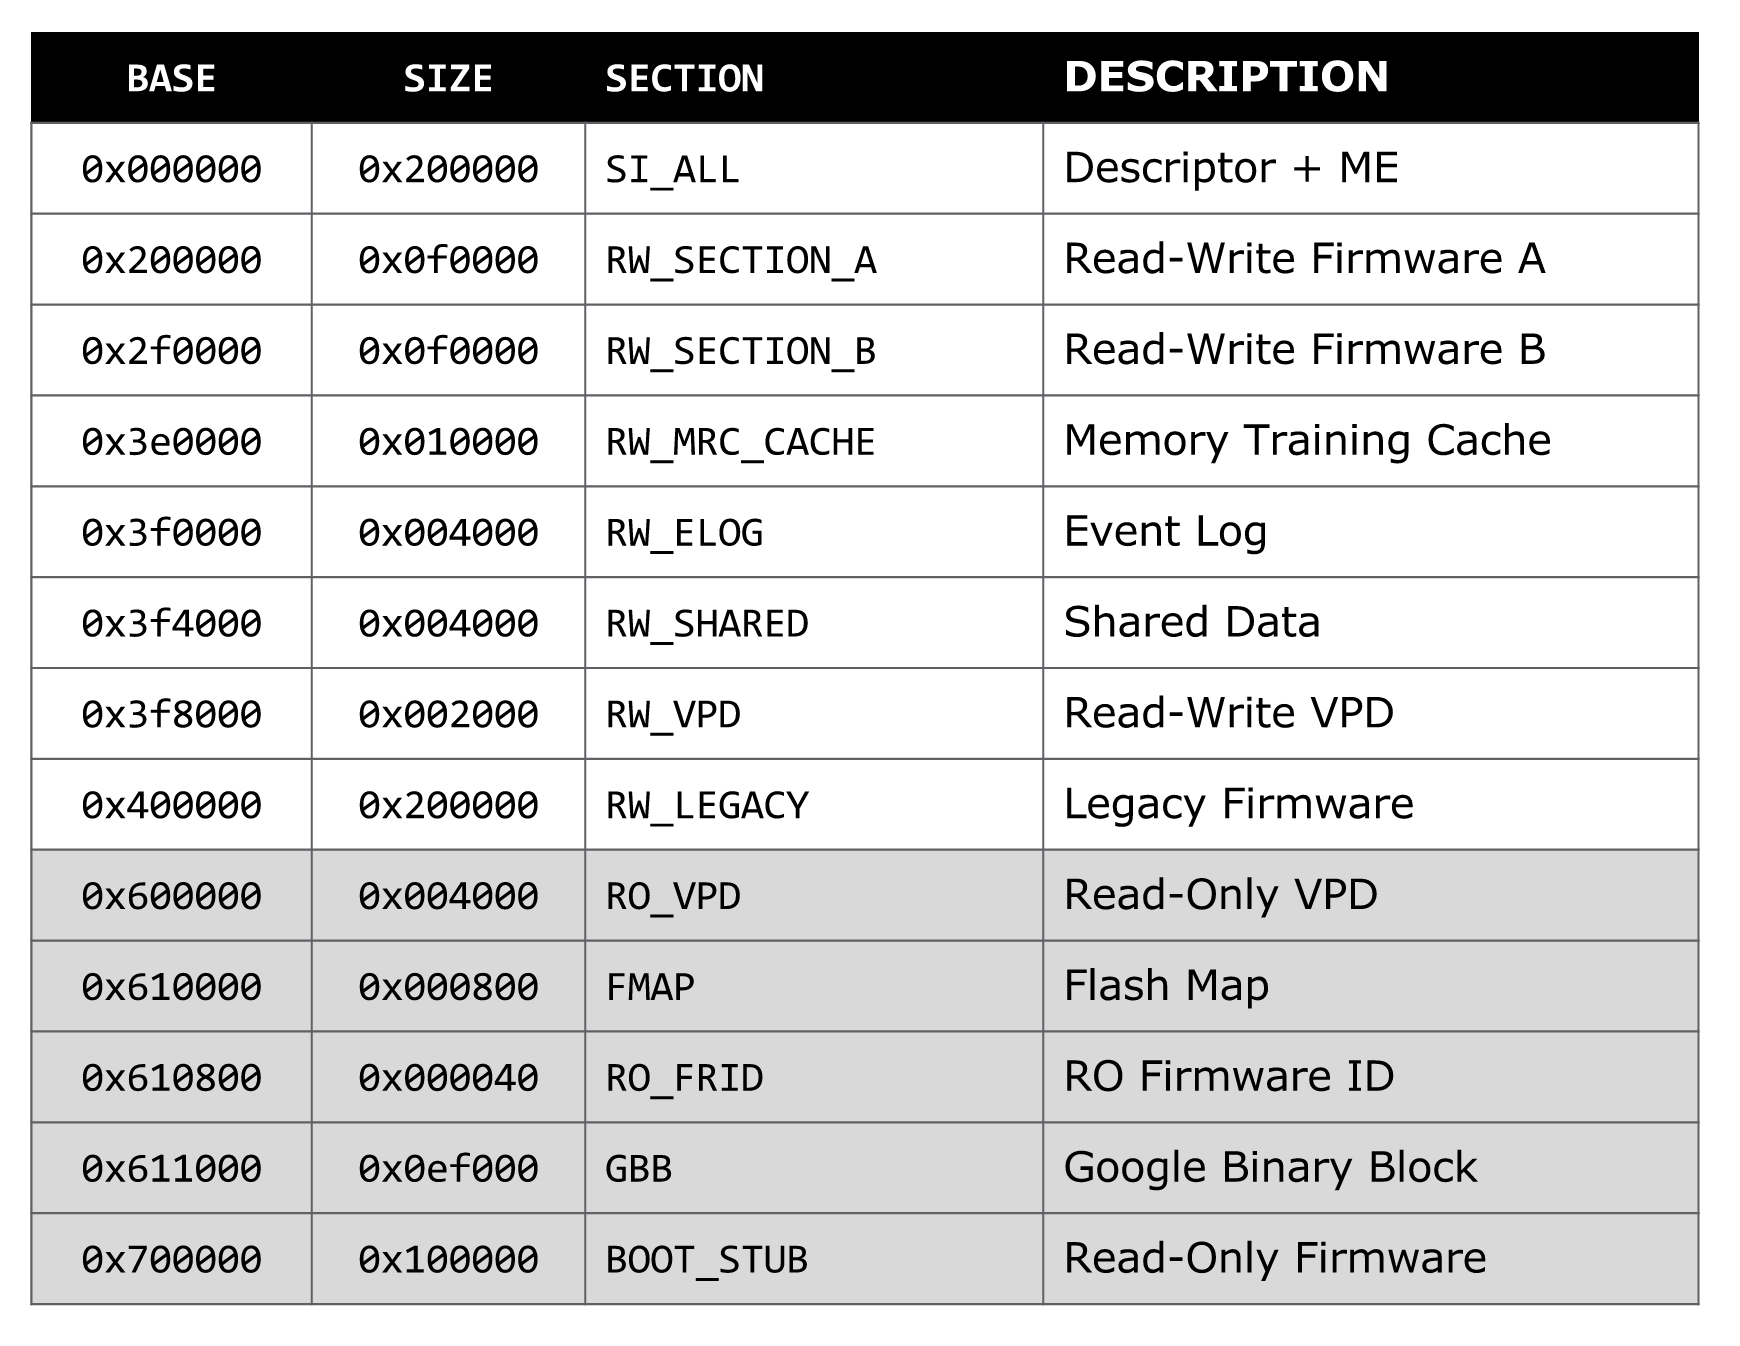
\includegraphics[width=0.8\linewidth]{fmap_locs.png}
  \caption[Chrome OS's Flash Map]{The Flash Map for Chrome OS's SPI Flash. The gray sections have been marked as Read Only~\cite{fw-summit}}
  \label{fig:fmap}
\end{figure}

\begin{figure}[!htbp]
  \centering
  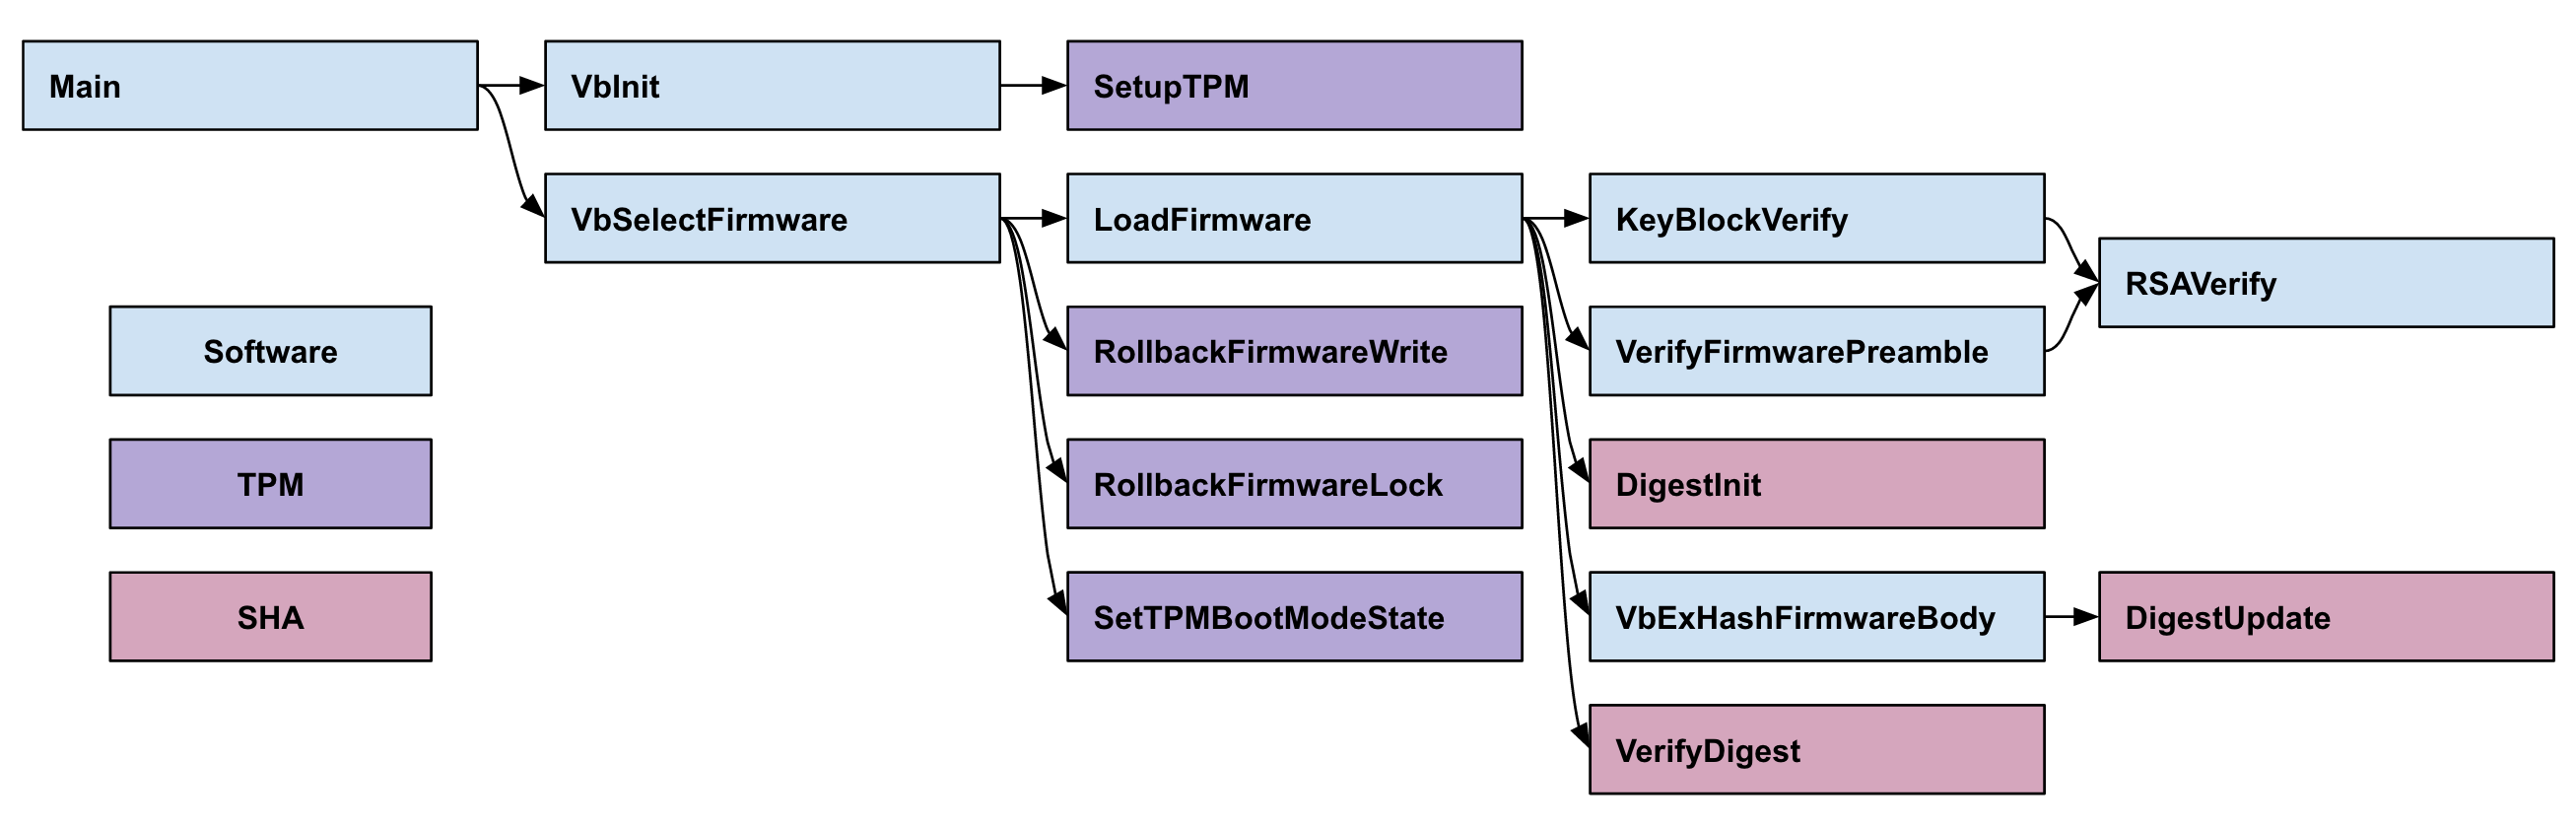
\includegraphics[width=1\linewidth]{full_flow.png}
  \caption{The full function call graph for Verified Boot}
  \label{fig:full_flow}
\end{figure}

\clearpage
\pagebreak

\begin{table}[!htbp]
    \centering
    \caption{All CBMC Tests}\label{all_results}
    \begin{tabular}{lrrrrr}
        \toprule
        test name & steps & VCCs & time (s) & memory (Mb) & sat/unsat  \\ \bottomrule
        \textbf{LoadFirmware}  &  & & & & \\
        Google Assertions & 6460 & 34 & 123 & 2312 & sat \\
        Rollback     & 4125 & 1 & 4 & 259 & unsat \\
        Rollback/rec & 4123 & 1 & 6 & 394 & sat \\
        Hash Failure & 4182 & 2 & 5 & 258 & unsat \\
        RSA  Failure & 4180 & 2 & 5 & 258 & unsat \\
        Array Accesses & 4130 & 57 & 126 & 2487 & unsat \\\midrule
        \textbf{LoadFirmware (malloc)}  &  & & & & \\
        Google Assertions & 6460 & 34 & 3799 & 60496 & unsat \\
        Rollback, Hash, RSA & 2858 & 6 & 3733 & 59874 & unsat \\\midrule
        \textbf{SelectFirmware}  &  & & & & \\
        TPM locking & 5269 & 6 & 2 & 164 & unsat \\
        LoadFirmware & 5264 & 2 & 3 & 164 & unsat \\
        Array Accesses & 5257 & 10 & 3 & 165 &  unsat \\\midrule
        \textbf{TPM}  &  & & & & \\
        Liveness & 20393 & 2220 & 387 & 15288 & unsat \\
        Error Handling & 20109 & 3 & 379 & 15281 & unsat \\
        Data Receive &  &  & & \\ \midrule
        \textbf{TLCL}  &  & & & & \\
        Error Handling & & & & \\
        SetupTPM & 613418 & 140 & 1674 & 6960 & unsat \\
        RollbackFirmwareWrite & 478639 & 108 & 952 & 5447 & unsat \\
        RollbackFirmwareLock & 17450 & 4 & 7 & 369 & unsat \\
        SetTPMBootModeState & 34621 & 8 & 11 & 397 & unsat \\ \midrule
    \end{tabular}
\end{table}
